


\newcommand{\pullnm}[3]{

\begin{frame}{Pulls for #3}
\begin{figure}
\includegraphics[width=\textwidth]{2020_05_19/antiSym_#1/pulls/#2.png}
\caption{Blue : $\pm 1$, Green : $\pm \frac{1}{\sqrt{N}}$}
\end{figure}
\end{frame}


\begin{frame}{Distributions for #3}
\begin{columns}
\begin{column}{0.33\textwidth}
\begin{figure}
\includegraphics[width=\textwidth]{2020_05_19/antiSym_#1/pulls/pulls/#2_00.png}
\caption{$C_{00}$}
\end{figure}
\hfill
\begin{figure}
\includegraphics[width=\textwidth]{2020_05_19/antiSym_#1/pulls/pulls/#2_01.png}
\caption{$C_{01}$}
\end{figure}
\hfill
\end{column}
\begin{column}{0.33\textwidth}
\begin{figure}
\includegraphics[width=\textwidth]{2020_05_19/antiSym_#1/pulls/pulls/#2_10.png}
\caption{$C_{10}$}
\end{figure}
\hfill
\begin{figure}
\includegraphics[width=\textwidth]{2020_05_19/antiSym_#1/pulls/pulls/#2_11.png}
\caption{$C_{11}$}
\end{figure}
\hfill

\end{column}
\begin{column}{0.33\textwidth}
\begin{figure}
\includegraphics[width=\textwidth]{2020_05_19/antiSym_#1/pulls/pulls/#2_02.png}
\caption{$C_{02}$}
\end{figure}
\hfill
\begin{figure}
\includegraphics[width=\textwidth]{2020_05_19/antiSym_#1/pulls/pulls/#2_20.png}
\caption{$C_{20}$}
\end{figure}
\hfill

\end{column}
\end{columns}
\end{frame}
}


\newcommand{\statusnm}[3]{
\begin{frame}{Statuses for #3}
\begin{figure}
\includegraphics[width=\textwidth]{2020_05_19/antiSym_#1/#2_Status.png}
\end{figure}
\end{frame}

}


\newcommand{\pullsnm}[2]{
\pullnm{#1}{Comb}{Combined Tags using #2}
\pullnm{#1}{KK}{$\KK$ Tag using #2}
\pullnm{#1}{Kspi0}{$\Kspiz$ Tag using #2}
\pullnm{#1}{Kppim}{$\Kppim$ Tag using #2}
\pullnm{#1}{Kmpip}{$\Kmpip$ Tag using #2}
\pullnm{#1}{Kspipi}{$\Kspipi$ Tag using #2}

}
\begin{frame}{Overview}
\begin{itemize}
\item Fixed the combined fitter object, the calculation of $\sum -2\log \mathcal{L}$ was not performed correctly - now it is.
\item Fitted the pull distribution with $N(\mu,\sigma)$ (as well as plotting the sample mean/deviation).
\end{itemize}
\end{frame}

\begin{frame}{Combined Log Liklihood}
With a single tag ($\KK$), the combined fit and the fit to $\KK$ should be identical for a given sample.
\begin{equation}
\sum \log \mathcal{L}_\text{tag} = \log \mathcal{L}_{KK}
\end{equation}
\end{frame}

\begin{frame}{Combined Log Liklihood}
\begin{columns}
\begin{column}{0.5\textwidth}
\begin{figure}
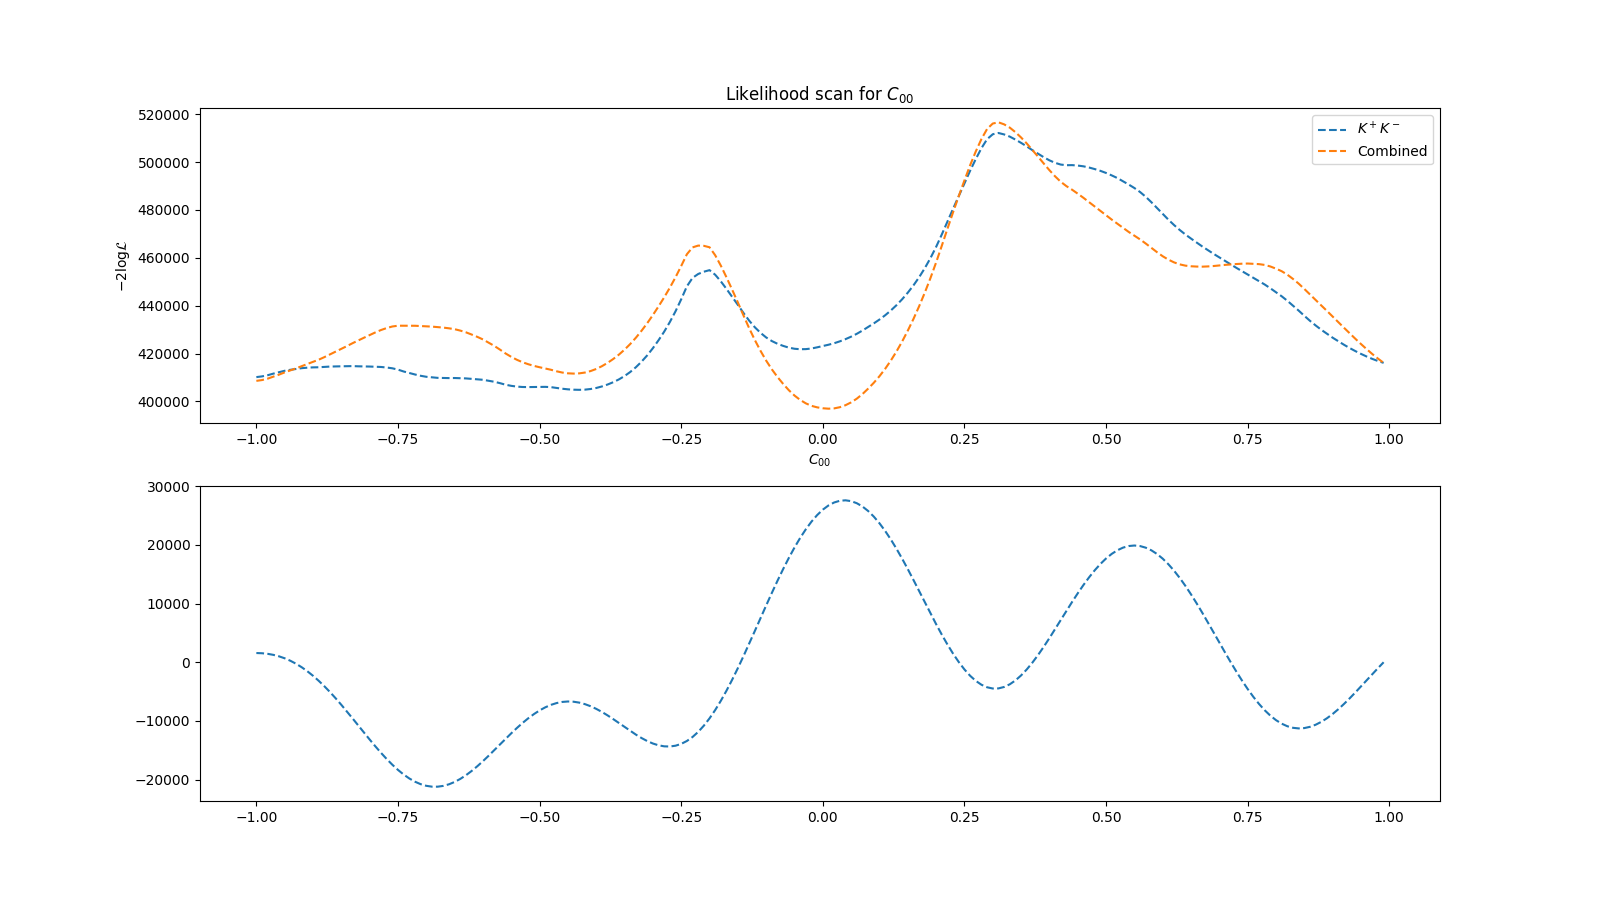
\includegraphics[width=\textwidth]{2020_05_19/combLL_test/old00/00.png}
\caption{Old method of calculating $\sum \log \mathcal{L}$}
\end{figure}
\hfill
\end{column}
\begin{column}{0.5\textwidth}
\begin{figure}
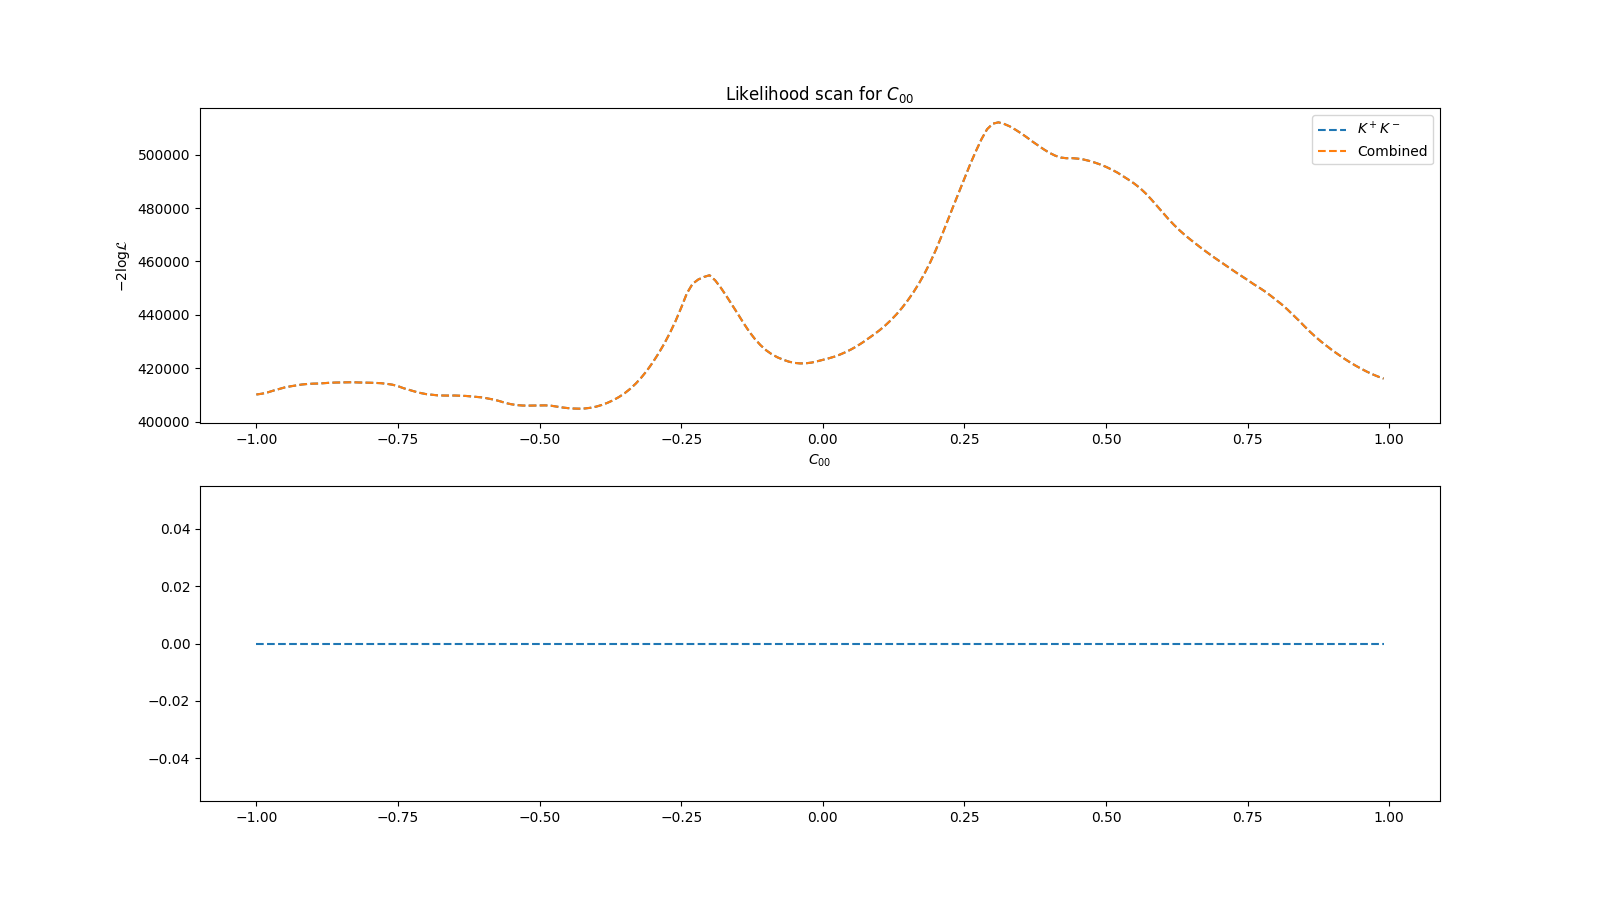
\includegraphics[width=\textwidth]{2020_05_19/combLL_test/new00/00.png}
\caption{New method of calculating $\sum \log \mathcal{L}$}
\end{figure}
\hfill
\end{column}
\end{columns}
\end{frame}

\begin{frame}{Antisymmetric simple polynomial}
\begin{center}
\begin{tabular}{|c|c|}
Coefficient & Polynomial \\ \hline
$C_{00}$ & $w_-$ \\
$C_{01}$ & $w_-^3$ \\
$C_{10}$ & $w_+ w_-$ \\
$C_{11}$ & $w_+ w_-^3$ \\
$C_{02}$ & $w_-^5$ \\
$C_{20}$ & $w_+^2 w_-$ \\ 
\end{tabular}
\end{center}
\end{frame}

\pullsnm{simple}{Antisymmetric simple polynomial}


\begin{frame}{Antisymmetric Legendre polynomial}
\begin{center}
\begin{tabular}{|c|c|}
Coefficient & Polynomial \\ \hline

$C_{00}$ & $w_-$ \\
$C_{01}$ & $\frac{1}{2} \left(5 w_-^3 - 5 w_-\right)$ \\
$C_{10}$ & $ w_+ w_-$ \\
$C_{11}$ & $ \frac{1}{2} w_+  \left(5 w_-^3 - 5 w_-\right)$\\
$C_{02}$ & $\frac{1}{8}\left(63 w_-^5 - 70 w_-^3 + 15 w_-\right)$ \\
$C_{20}$ & $\frac{1}{2} \left(3 w_+^2 - 1\right) w_-$

\end{tabular}
\end{center}
\end{frame}

\pullsnm{legendre}{Antisymmetric legendre polynomial}

\begin{frame}{Antisymmetric chebyshev polynomial}
\begin{center}
\begin{tabular}{|c|c|}
Coefficient & Polynomial \\ \hline

$C_{00}$ & $w_-$ \\
$C_{01}$ & $4 w_-^3 - 3 w_-$ \\
$C_{10}$ & $ w_+ w_-$ \\
$C_{11}$ & $ w_+ \left(4 w_-^3 - 3 w_-\right)$\\
$C_{02}$ & $16 w_-^5 - 20 w_-^3 + 5 w_-$ \\
$C_{20}$ & $\left(2 w_+^2 - 1\right) w_-$

\end{tabular}
\end{center}
\end{frame}

\pullsnm{chebyshev}{Antisymmetric chebyshev polynomial}

\begin{frame}{Next Steps}
\begin{itemize}
\item Increase statistics on the pull study to $N=100$
\end{itemize}
\end{frame}


